Photoelectron multiplier tube, PMT, is one of the most used photosensors in nuclear physics during last decades. Its main objective, like all photosensors, is to detect the scintillating photons that reach its sensible part and covert it in an electronic signal large enough to be measured. 

In Figure \ref{fig:SchemePMT} there is a schematic drawing where it can be appreciate the PMT components and how it works. As it can be seen in this figure, the electrons created in the photocathode (electronic signal) need to travel in the medium so, to increase the amount of conserved electrons, it is needed to work inside a vacuum tube. Therefore, the PMT consists of a vacuum tube that has a glass window through which photons can penetrate.  

\begin{figure}[htbp]
\centering
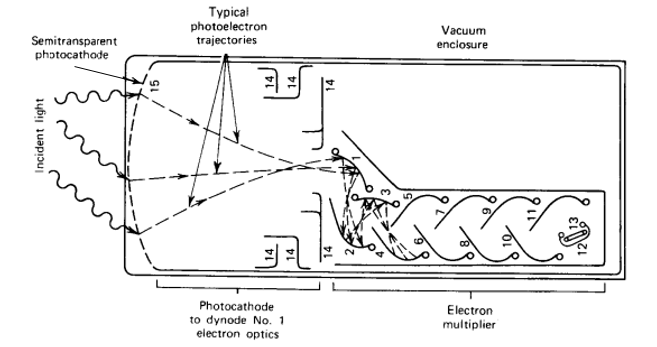
\includegraphics[scale=0.6]{3DesignPrinciples/32Tritium_detector/PMTschematic.png}
\caption{Scheme of a PMT.\label{fig:SchemePMT}~\cite{Knoll}}
\end{figure}

The way in which PMT achieves their aim of detecting scintillating photons happen inside this vacuum tube and it is based in two different phases:

\begin{itemize}
\item{} First, the PMT convert photons that reach its sensible part in electrons, called photoelectrons, with some probability through photoelectric effect. This sensitive part is the photocathode, which consists of a thin layer (thickness of the order of nanometers) deposited on the inner surface of the PMT windows. The material of the photocathode is chosen to increase the probability of producing photoelectric effect with the scintillating photons. The PMTs used in TRITIUM experiment are the model R8520-406 from Hammatsu \cite{DataSheetPMTs} and the material of its photocathode is Bialkali\footnote{The bialkali material is based on the elements $\ce{^{121}_{51}Sb}$, $\ce{^{85}_{37}Rb}$ and $\ce{^{132}_{55}Cs}$}.

The response of the PMT at long wavelengths is limited mainly because the photon does not have enough energy to produce a photoelectric effect or the emitted photoelectron does not have enough energy to overcome the material-vacuum interface. The response of the PMT at short wavelengths is limited mainly due to absorption in the window material, quartz in our case. Due to both reasons, the response of the PMT will have a strong dependence with the energy of the photon and it's commonly expressed in the quantum efficiency (QE) spectrum which is the quotient between the number of photoelectrons produced at the cathode of the PMT and the number of photons reaching it. For PMTs used in TRITIUM experiment, it is showed in Figure \ref{fig:QuantumEfficiencyPMT}.

\begin{figure}[htbp]
\centering
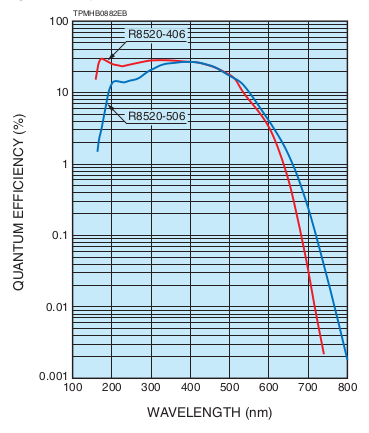
\includegraphics[scale=0.5]{3DesignPrinciples/32Tritium_detector/QuantumEfficiencyPMT.png}
\caption{Quantum efficiency spectrum for the PMT used (R8520-406).\label{fig:QuantumEfficiencyPMT}~\cite{DataSheetPMTs}}
\end{figure}

The maximum values of the PMT quantum efficiency is commonly between $20\%$ and $30\%$ \cite{Knoll} (a little bit less than $30\%$ for the PMTs used). Comparing the emission spectrum of the scintillating fibers used, Figure \ref{fig:EmissionSpectrumFibers}, and the quantum efficiency spectrum of the PMTs used, Figure \ref{fig:QuantumEfficiencyPMT}, it can be seen that both are approximately in the same energy range. In addition, the position of both the peaks are very close, $435~\nm$ for fibers and $420~\nm$ for PMTs. As said before, it means that overall efficiency is optimized.

\item{} Next, because of the reason that the number of photoelectrons in the photocatode is very small, a electron multiplication stage is needed to achieve a large enough electronic signal to be processed by the electronic system. 

This stage is based on three elements, focusing electrodes, dynodes and anode: They are metallic sheet with a shape and position that are designed to optimize the collection and multiplication of electrons. A high voltage (HV) is applied to the PMT which are distributed between all this elements, including the photocathode. It is distributed in a increasing voltage way in order to attract and accelerate the electrons. An electronic circuit is used to make this distribution and it can be fed with positive voltage, ground in the photocathode, which could be interesting for measuring PMT currents, or negative voltage, ground in the anode, the response of which is faster. The comercial electronic circuits of Hammatsu are showed in Figure \ref{fig:VoltageDividerCircuit}.

\begin{figure}[h]
\centering
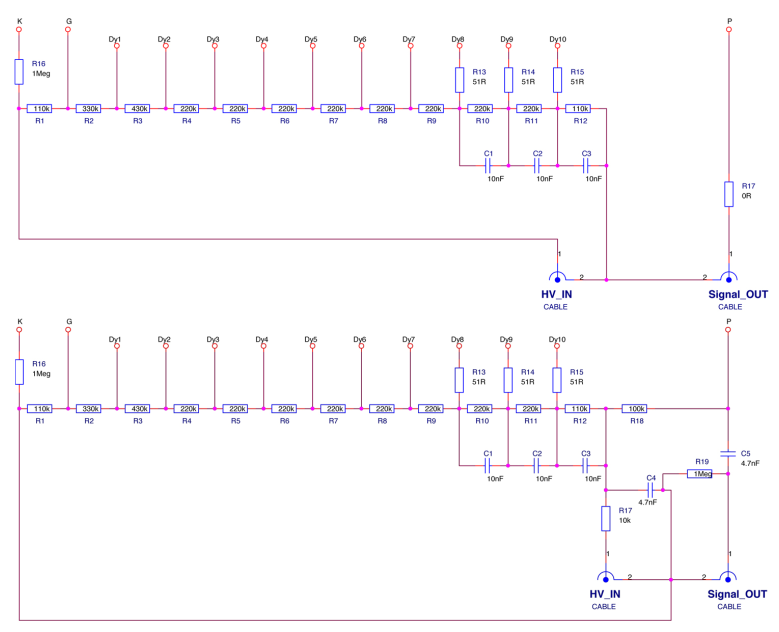
\includegraphics[scale=0.5]{3DesignPrinciples/32Tritium_detector/VoltageDividerPMT.png}
\caption{Hamamatsu commercial voltage divider electronic circuit. Upper circuit with negative supply and lower circuit with positive supply.\label{fig:VoltageDividerCircuit}~\cite{DataSheetPMTs}}
\end{figure}

%The electronic circuit that can be supplied with negative voltage is faster due to the ausence of the capacitances C4 and C5, but the other circuit, supplied with positive voltage, can be interesting for other tasks like the measurement of PMT currents. We will use both, depends on the objective of the study.

Focusing electrodes are used to guide the photoelectrons to the first dinode. Therefore, they have an collection efficiency (CE) that is defined as the quotient between the number of photoelectrons reaching the first dinode and the number of photoelectrons leaving the photocathode and its value is around $80\%$ for PMTs.

The dynodes is the part where the multiplication takes place. They have different voltage between each dynode in order to accelerate the electrons and produce their multiplication. The multiplication factor of each dynode, $\delta$, is commonly around 5 and it has a strongly dependence with the HV. Therefore, guessing the same gain for all dynodes, the overall gain of the PMT with N dynodes is:

\begin{equation}
G = CE\cdot{} \delta^N~\cite{Knoll}
\label{eq:PMTGain}
\end{equation}

Using the numerical values previously mentioned, the overall gain of a general PMT will be of the order of $10^6$ and, as it has been mentioned, this value depends strongly on the used HV.

It has to be taken into account that the multiplication stage add a uncertainty in the measurement. Due to that, it could be interesting to work without gain in some situations, for example to count the number of photons that reach the PMT. It can be done with a small modification of the electronic voltage divider circuit \ref{fig:VoltageDividerCircuit} which, As it will be shown in section \ref{subsubsec:PMTsElectronicalSystem}, it consists of short-circuiting all the dindes and the anode and collect the signal in the photocatode. This special setup will be used for the fiber characterization, section \ref{subsec:CharacterizationFibers}.

Finally, the anode is the point where the collection of all the electrons produced takes place and it is the one that gives rise to the output signal of the PMTs.

\end{itemize}

The output signal of a PMT has a spread of the order of tens of nanoseconds and its multiplication can be described as a Poisson statistical process, so, for each electron in the first dinode, G new electrons will be created with a variance of $\sqrt{G}$.

The output signal of a PMT is linear with the number of photons that reach its sensitive part up to a limit, where saturation takes place and the linearity is lost. This limit depends on the PMT model.

Finally, It is important to take into account that the photocathode can emit electrons with an origin that doesn't belong to the scintillation light. This signal, which is named dark current, can  happen due to several reasons like cosmic radiation, light from environment or thermoionic emission (the dominant) and, for the PMTs used, this value is around $2~\nano\ampere$ according to its data sheet.

The calibration of the most important (for TRITIUM experiment) of the PMTs used, which are dark current, gain for several HV and quantum efficiency,  have been done at IFIC in the framework of NEXT experiment \cite{CalibrationPMTsNEXT}. 